\begin{pastexam}[label={px:ncku-111-prog-02}]{成大資訊聯招 111 學年度 第 2 題}
（單選）

\textbf{[2\%]} We rely on the tree data structure to represent a set of elements. Two elements are in the same set if they share the common root. Given two sets as follows, which is true if we union the two sets? Assume the union follows the height union rule.

\begin{center}
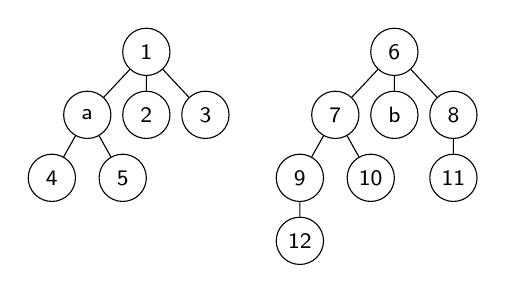
\begin{tikzpicture}[x=0.75cm,y=0.8cm,v/.style={circle,draw,inner sep=0pt,minimum size=6mm,font=\footnotesize\sffamily},s/.style={v,fill=black!25}]
\node[v] (n1) at (2,0) {1};
\node[v] (na) at (1,-1) {a};
\node[v] (n2) at (2,-1) {2};
\node[v] (n3) at (3,-1) {3};
\node[v] (n4) at (0.4,-2) {4};
\node[v] (n5) at (1.6,-2) {5};
\node[v] (n6) at (6.2,0) {6};
\node[v] (n7) at (5.2,-1) {7};
\node[v] (nb) at (6.2,-1) {b};
\node[v] (n8) at (7.2,-1) {8};
\node[v] (n9) at (4.6,-2) {9};
\node[v] (n10) at (5.8,-2) {10};
\node[v] (n11) at (7.2,-2) {11};
\node[v] (n12) at (4.6,-3) {12};
\draw (n1)--(na) (n1)--(n2) (n1)--(n3) (na)--(n4) (na)--(n5) (n6)--(n7) (n6)--(nb) (n6)--(n8) (n7)--(n9) (n7)--(n10) (n8)--(n11) (n9)--(n12);
\end{tikzpicture}
\end{center}

(A)
\begin{center}
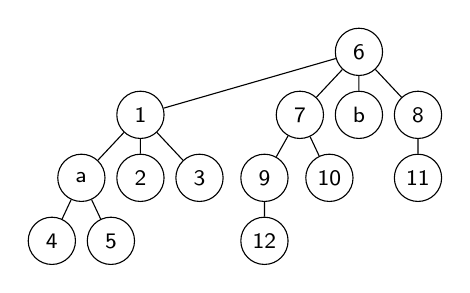
\begin{tikzpicture}[x=0.75cm,y=0.8cm,v/.style={circle,draw,inner sep=0pt,minimum size=6mm,font=\footnotesize\sffamily},s/.style={v,fill=black!25}]
\node[v] (n6) at (5.2,0) {6};
\node[v] (n1) at (1.5,-1) {1};
\node[v] (n7) at (4.2,-1) {7};
\node[v] (nb) at (5.2,-1) {b};
\node[v] (n8) at (6.2,-1) {8};
\node[v] (na) at (0.5,-2) {a};
\node[v] (n2) at (1.5,-2) {2};
\node[v] (n3) at (2.5,-2) {3};
\node[v] (n9) at (3.6,-2) {9};
\node[v] (n10) at (4.7,-2) {10};
\node[v] (n11) at (6.2,-2) {11};
\node[v] (n4) at (0,-3) {4};
\node[v] (n5) at (1,-3) {5};
\node[v] (n12) at (3.6,-3) {12};
\draw (n6)--(n1) (n6)--(n7) (n6)--(nb) (n6)--(n8) (n1)--(na) (n1)--(n2) (n1)--(n3) (na)--(n4) (na)--(n5) (n7)--(n9) (n7)--(n10) (n9)--(n12) (n8)--(n11);
\end{tikzpicture}
\end{center}

(B)
\begin{center}
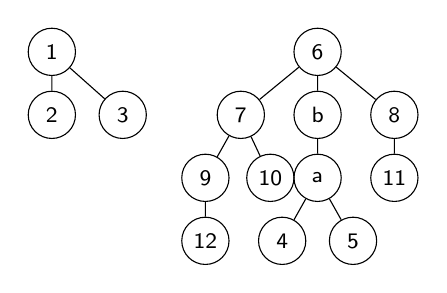
\begin{tikzpicture}[x=0.75cm,y=0.8cm,v/.style={circle,draw,inner sep=0pt,minimum size=6mm,font=\footnotesize\sffamily},s/.style={v,fill=black!25}]
\node[v] (n1) at (0,0) {1};
\node[v] (n2) at (0,-1) {2};
\node[v] (n3) at (1.2,-1) {3};
\node[v] (n6) at (4.5,0) {6};
\node[v] (n7) at (3.2,-1) {7};
\node[v] (nb) at (4.5,-1) {b};
\node[v] (n8) at (5.8,-1) {8};
\node[v] (n9) at (2.6,-2) {9};
\node[v] (n10) at (3.7,-2) {10};
\node[v] (na) at (4.5,-2) {a};
\node[v] (n11) at (5.8,-2) {11};
\node[v] (n12) at (2.6,-3) {12};
\node[v] (n4) at (3.9,-3) {4};
\node[v] (n5) at (5.1,-3) {5};
\draw (n1)--(n2) (n1)--(n3) (n6)--(n7) (n6)--(nb) (n6)--(n8) (n7)--(n9) (n7)--(n10) (nb)--(na) (n8)--(n11) (n9)--(n12) (na)--(n4) (na)--(n5);
\end{tikzpicture}
\end{center}

(C)
\begin{center}
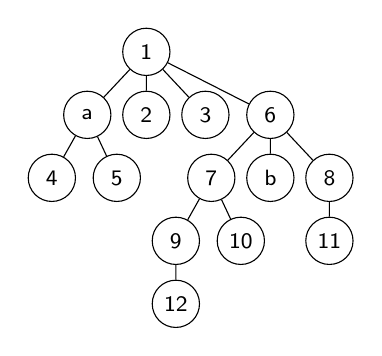
\begin{tikzpicture}[x=0.75cm,y=0.8cm,v/.style={circle,draw,inner sep=0pt,minimum size=6mm,font=\footnotesize\sffamily},s/.style={v,fill=black!25}]
\node[v] (n1) at (1.8,0) {1};
\node[v] (na) at (0.8,-1) {a};
\node[v] (n2) at (1.8,-1) {2};
\node[v] (n3) at (2.8,-1) {3};
\node[v] (n6) at (3.9,-1) {6};
\node[v] (n4) at (0.2,-2) {4};
\node[v] (n5) at (1.3,-2) {5};
\node[v] (n7) at (2.9,-2) {7};
\node[v] (nb) at (3.9,-2) {b};
\node[v] (n8) at (4.9,-2) {8};
\node[v] (n9) at (2.3,-3) {9};
\node[v] (n10) at (3.4,-3) {10};
\node[v] (n11) at (4.9,-3) {11};
\node[v] (n12) at (2.3,-4) {12};
\draw (n1)--(na) (n1)--(n2) (n1)--(n3) (n1)--(n6) (na)--(n4) (na)--(n5) (n6)--(n7) (n6)--(nb) (n6)--(n8) (n7)--(n9) (n7)--(n10) (n8)--(n11) (n9)--(n12);
\end{tikzpicture}
\end{center}

(D)
\begin{center}
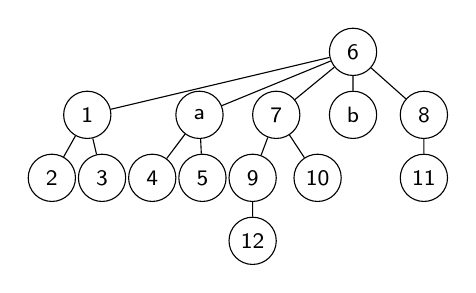
\begin{tikzpicture}[x=0.75cm,y=0.8cm,v/.style={circle,draw,inner sep=0pt,minimum size=6mm,font=\footnotesize\sffamily},s/.style={v,fill=black!25}]
\node[v] (n6) at (5.2,0) {6};
\node[v] (n1) at (0.7,-1) {1};
\node[v] (na) at (2.6,-1) {a};
\node[v] (n7) at (3.9,-1) {7};
\node[v] (nb) at (5.2,-1) {b};
\node[v] (n8) at (6.4,-1) {8};
\node[v] (n2) at (0.1,-2) {2};
\node[v] (n3) at (0.95,-2) {3};
\node[v] (n4) at (1.8,-2) {4};
\node[v] (n5) at (2.65,-2) {5};
\node[v] (n9) at (3.5,-2) {9};
\node[v] (n10) at (4.6,-2) {10};
\node[v] (n11) at (6.4,-2) {11};
\node[v] (n12) at (3.5,-3) {12};
\draw (n6)--(n1) (n6)--(na) (n6)--(n7) (n6)--(nb) (n6)--(n8) (n1)--(n2) (n1)--(n3) (na)--(n4) (na)--(n5) (n7)--(n9) (n7)--(n10) (n8)--(n11) (n9)--(n12);
\end{tikzpicture}
\end{center}

(E) None.\end{pastexam}

\begin{pastsoln}
答案：(A)。

\textbf{依高度合併}（union by height，資結書第~13.2.2~節）：合併兩棵樹時，讓\textbf{高度較小}那棵的
根成為高度較大那棵的根的子節點；兩棵一樣高時任選一個當根，新樹高度加 $1$。 這樣合併後的高度只有在兩棵
一樣高時才會增加，樹高保持在 $O(\log n)$。 合併只改一個指標（矮的那棵的根的父指標），兩棵樹內部的
形狀都不動。

\textbf{兩棵樹的高度}（以邊數計）：
\begin{itemize}
\item 以 $1$ 為根的樹：最長的路是 $1 \to a \to 4$（或 $5$），高度 $2$。
\item 以 $6$ 為根的樹：最長的路是 $6 \to 7 \to 9 \to 12$，高度 $3$。
\end{itemize}
$1$ 那棵比較矮，所以 $1$ 成為 $6$ 的子節點，$1$ 的整棵子樹（$a$、$2$、$3$、$4$、$5$）原封不動跟著
過去。 合併後高度是 $\max(3, 2 + 1) = 3$，沒有增加。

逐項檢查：
\begin{itemize}
\item (A)：$6$ 是根，$1$ 接在 $6$ 下面，兩棵原本的形狀都沒變。 正確。
\item (B)：$a$ 被搬到 $b$ 下面，$1$ 只剩 $2$、$3$，而且 $1$ 和 $6$ 沒有連在一起，還是兩個集合。
合併不會拆開原本的樹，錯。
\item (C)：$6$ 接到 $1$ 下面，是把高的那棵接到矮的下面，高度變成 $4$，違反依高度合併的規則，錯。
\item (D)：$1$ 的子節點 $a$ 被拉到 $6$ 底下，像是做了路徑壓縮之類的重排；單純的合併不會改變 $1$ 的
子樹，錯。
\item (E)：(A) 正確，所以不選。
\end{itemize}
\end{pastsoln}
